% Created 2021-10-29 Fri 13:49
% Intended LaTeX compiler: pdflatex
\documentclass{scrartcl}
\usepackage[utf8]{inputenc}
\usepackage[T1]{fontenc}
\usepackage{fontspec}
\usepackage{graphicx}
\usepackage{grffile}
\usepackage{longtable}
\usepackage{wrapfig}
\usepackage{rotating}
\usepackage[normalem]{ulem}
\usepackage{amsmath}
\usepackage{textcomp}
\usepackage{amssymb}
\usepackage{capt-of}
\usepackage[dvipsnames]{xcolor}
\usepackage[colorlinks=true, linkcolor=Blue, citecolor=BrickRed, urlcolor=PineGreen]{hyperref}
\usepackage{indentfirst}
% features: (custom-font acronym underline italic-quotes par-sep alegreya-typeface image)
\usepackage[osf]{Alegreya}
\usepackage{AlegreyaSans}
\usepackage[scale=0.88]{sourcecodepro}

\newcommand{\acr}[1]{\protect\textls*[110]{\scshape #1}}
\newcommand{\acrs}{\protect\scalebox{.91}[.84]\hspace{0.15ex}s}
\usepackage[normalem]{ulem}
\renewcommand{\quote}{\list{}{\rightmargin\leftmargin}\item\relax\em}

\setlength{\parskip}{\baselineskip}
\setlength{\parindent}{0pt}

\usepackage{graphicx}
% end features

%% make document follow Emacs theme

\definecolor{obg}{HTML}{ffffff}
\definecolor{ofg}{HTML}{000000}

\pagecolor{obg}
\color{ofg}

% list labels

\definecolor{itemlabel}{HTML}{4078f2}

\renewcommand{\labelitemi}{\textcolor{itemlabel}{\textbullet}}
\renewcommand{\labelitemii}{\textcolor{itemlabel}{\normalfont\bfseries \textendash}}
\renewcommand{\labelitemiii}{\textcolor{itemlabel}{\textasteriskcentered}}
\renewcommand{\labelitemiv}{\textcolor{itemlabel}{\textperiodcentered}}

\renewcommand{\labelenumi}{\textcolor{itemlabel}{\theenumi.}}
\renewcommand{\labelenumii}{\textcolor{itemlabel}{(\theenumii)}}
\renewcommand{\labelenumiii}{\textcolor{itemlabel}{\theenumiii.}}
\renewcommand{\labelenumiv}{\textcolor{itemlabel}{\theenumiv.}}

% structural elements

\definecolor{documentTitle}{HTML}{a626a4}
\definecolor{documentInfo}{HTML}{a626a4}
\definecolor{level1}{HTML}{e45649}
\definecolor{level2}{HTML}{da8548}
\definecolor{level3}{HTML}{b751b6}
\definecolor{level4}{HTML}{6f99f5}
\definecolor{level5}{HTML}{bc5cba}
\definecolor{level6}{HTML}{9fbbf8}
\definecolor{level7}{HTML}{d292d1}
\definecolor{level8}{HTML}{d8e4fc}

\addtokomafont{title}{\color{documentTitle}}
\addtokomafont{author}{\color{documentInfo}}
\addtokomafont{date}{\color{documentInfo}}
\addtokomafont{section}{\color{level1}}
\newkomafont{sectionprefix}{\color{level1}}
\addtokomafont{subsection}{\color{level2}}
\newkomafont{subsectionprefix}{\color{level2}}
\addtokomafont{subsubsection}{\color{level3}}
\newkomafont{subsubsectionprefix}{\color{level3}}
\addtokomafont{paragraph}{\color{level4}}
\newkomafont{paragraphprefix}{\color{level4}}
\addtokomafont{subparagraph}{\color{level5}}
\newkomafont{subparagraphprefix}{\color{level5}}

% textual elements

\definecolor{link}{HTML}{4078f2}
\definecolor{cite}{HTML}{4aa8b0}
\definecolor{itemlabel}{HTML}{4078f2}
\definecolor{code}{HTML}{da8548}
\definecolor{verbatim}{HTML}{50a14f}

\renewcommand{\labelitemi}{\textcolor{itemlabel}{\textbullet}}
\renewcommand{\labelitemii}{\textcolor{itemlabel}{\normalfont\bfseries \textendash}}
\renewcommand{\labelitemiii}{\textcolor{itemlabel}{\textasteriskcentered}}
\renewcommand{\labelitemiv}{\textcolor{itemlabel}{\textperiodcentered}}

\renewcommand{\labelenumi}{\textcolor{itemlabel}{\theenumi.}}
\renewcommand{\labelenumii}{\textcolor{itemlabel}{(\theenumii)}}
\renewcommand{\labelenumiii}{\textcolor{itemlabel}{\theenumiii.}}
\renewcommand{\labelenumiv}{\textcolor{itemlabel}{\theenumiv.}}

\DeclareTextFontCommand{\texttt}{\color{code}\ttfamily}
\makeatletter
\def\verbatim@font{\color{verbatim}\normalfont\ttfamily}
\makeatother

% code blocks

\definecolor{codebackground}{HTML}{f6f6f6}
\colorlet{EFD}{ofg}
\definecolor{codeborder}{HTML}{f0f0f0}

%% end customisations

\author{Shaurya Singh}
\date{\today}
\title{IRR 1 Bibliography}
\colorlet{greenyblue}{blue!70!green}
\colorlet{blueygreen}{blue!40!green}
\providecolor{link}{named}{greenyblue}
\providecolor{cite}{named}{blueygreen}
\hypersetup{
  pdfauthor={Shaurya Singh},
  pdftitle={IRR 1 Bibliography},
  pdfkeywords={},
  pdfsubject={},
  pdfcreator={Emacs 29.0.50 (Org mode 9.5)},
  pdflang={English},
  breaklinks=true,
  colorlinks=true,
  linkcolor=,
  urlcolor=link,
  citecolor=cite
}
\urlstyle{same}
\begin{document}

\maketitle
\setcounter{tocdepth}{2}
\tableofcontents

\subsection{Group Question (WIP)}
\label{sec:orge3167f8}
Does the caffeine in coffee present health risks for middle aged people in America?
\subsection{Lens/Individual Question}
\label{sec:org5abcebc}
What is the influence of adolescent coffee consumption and coffee culture on future risk of type 2 diabetes mellitus in middle aged men and women?

\section{Article 1: Adolescent dairy product consumption and risk of type 2 diabetes in middle-aged women}
\label{sec:org5d655c9}
\subsection{PDF}
\label{sec:orga416fc2}
\begin{center}
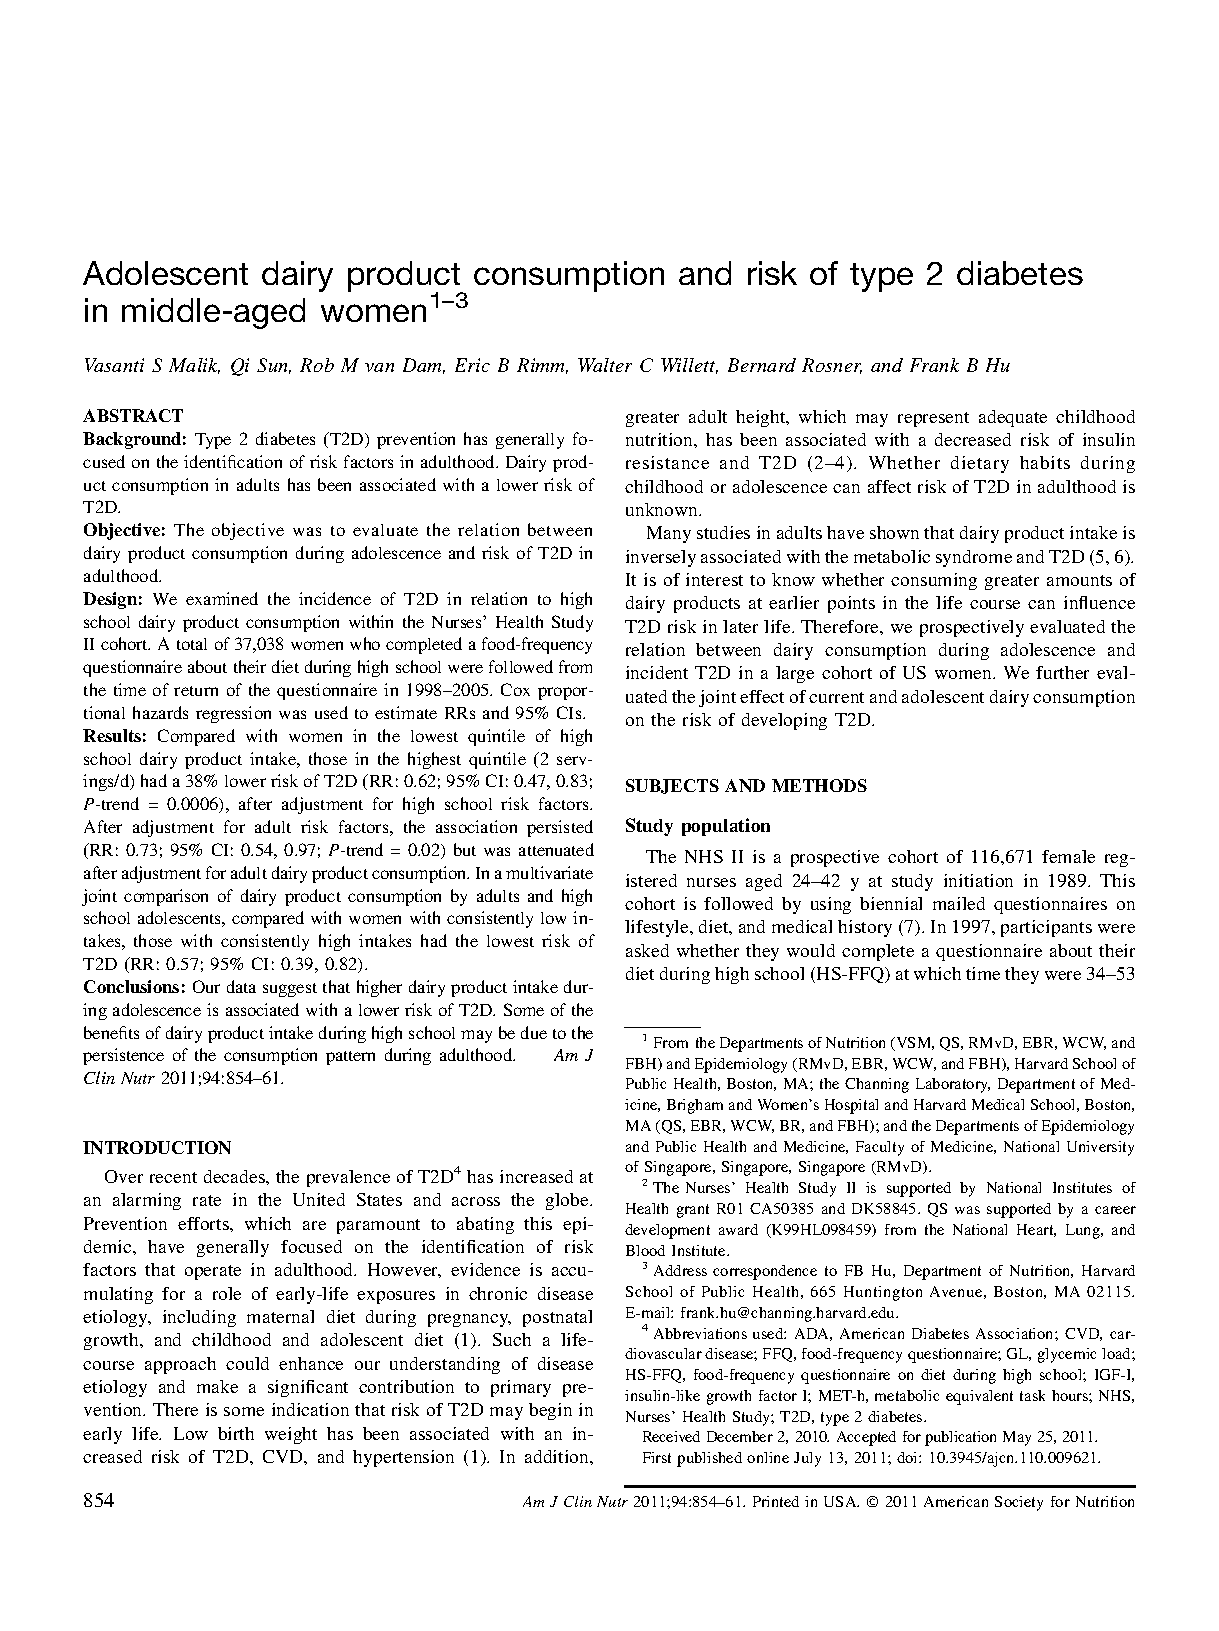
\includegraphics[width=.9\linewidth]{./citations/AdolescentDairyConsumption.pdf}
\end{center}
\subsection{MLA Citation}
\label{sec:org23ae21b}
\begin{quote}
Malik, V. S., et al. “Adolescent Dairy Product Consumption and Risk of Type 2 Diabetes in Middle-Aged Women.” American Journal of Clinical Nutrition, vol. 94, no. 3, Sept. 2011, pp. 854–61. DOI.org (Crossref), \url{https://doi.org/10.3945/ajcn.110.009621}.
\end{quote}
\subsection{A brief summary of the text}
\label{sec:org1581e2c}
The text examines the effect of adolescent dairy consumption on the future risk of type 2 diabetes, specifically on women. It does this on a global scale, providing statistics on the effect of dairy on adult height growth, insulin resistance, and resulting CI's at later ages. The study concludes that higher diary reduces the chances of T2D in adulthood.
\subsection{Comment on the authority or credibility of the author;}
\label{sec:org29fed60}
All the authors are credible. They are experts in their various fields. The article itself is published on pubmed NCBI, a non-profit and well known peer reviewed journal.
\subsection{Comment on strengths and weaknesses of their argument;}
\label{sec:org0f1b969}
The study is very in depth, has taken care of any external factors they needed to control, and presents their data in a well thought out way. However, the sample size could be more descriptive (the research only gives the number of women, not where they were from etc.)
\subsection{The author’s point of view; and}
\label{sec:orgae33f3d}
The author is a neutral writer, in that this is a purely informative piece
\subsection{How the text relates to your question or thesis.}
\label{sec:org0165600}
The text identifies dairy intake in adolescence and relates it risk of diabetes in elder women. Since coffee is a subset of dairy, the benefits of dairy apply to coffee as well
\section{Article 2: Influence of Adolescent and Maternal Coffee Consumption on Risk of Obesity and Type 2 Diabetes Mellitus in Middle-Aged Women and Their Offspring: Results from Two Prospective Cohort Studies in the United States}
\label{sec:orgdab8b7f}
\subsection{PDF\hfill{}\textsc{ATTACH}}
\label{sec:orgb153ab8}
\begin{center}
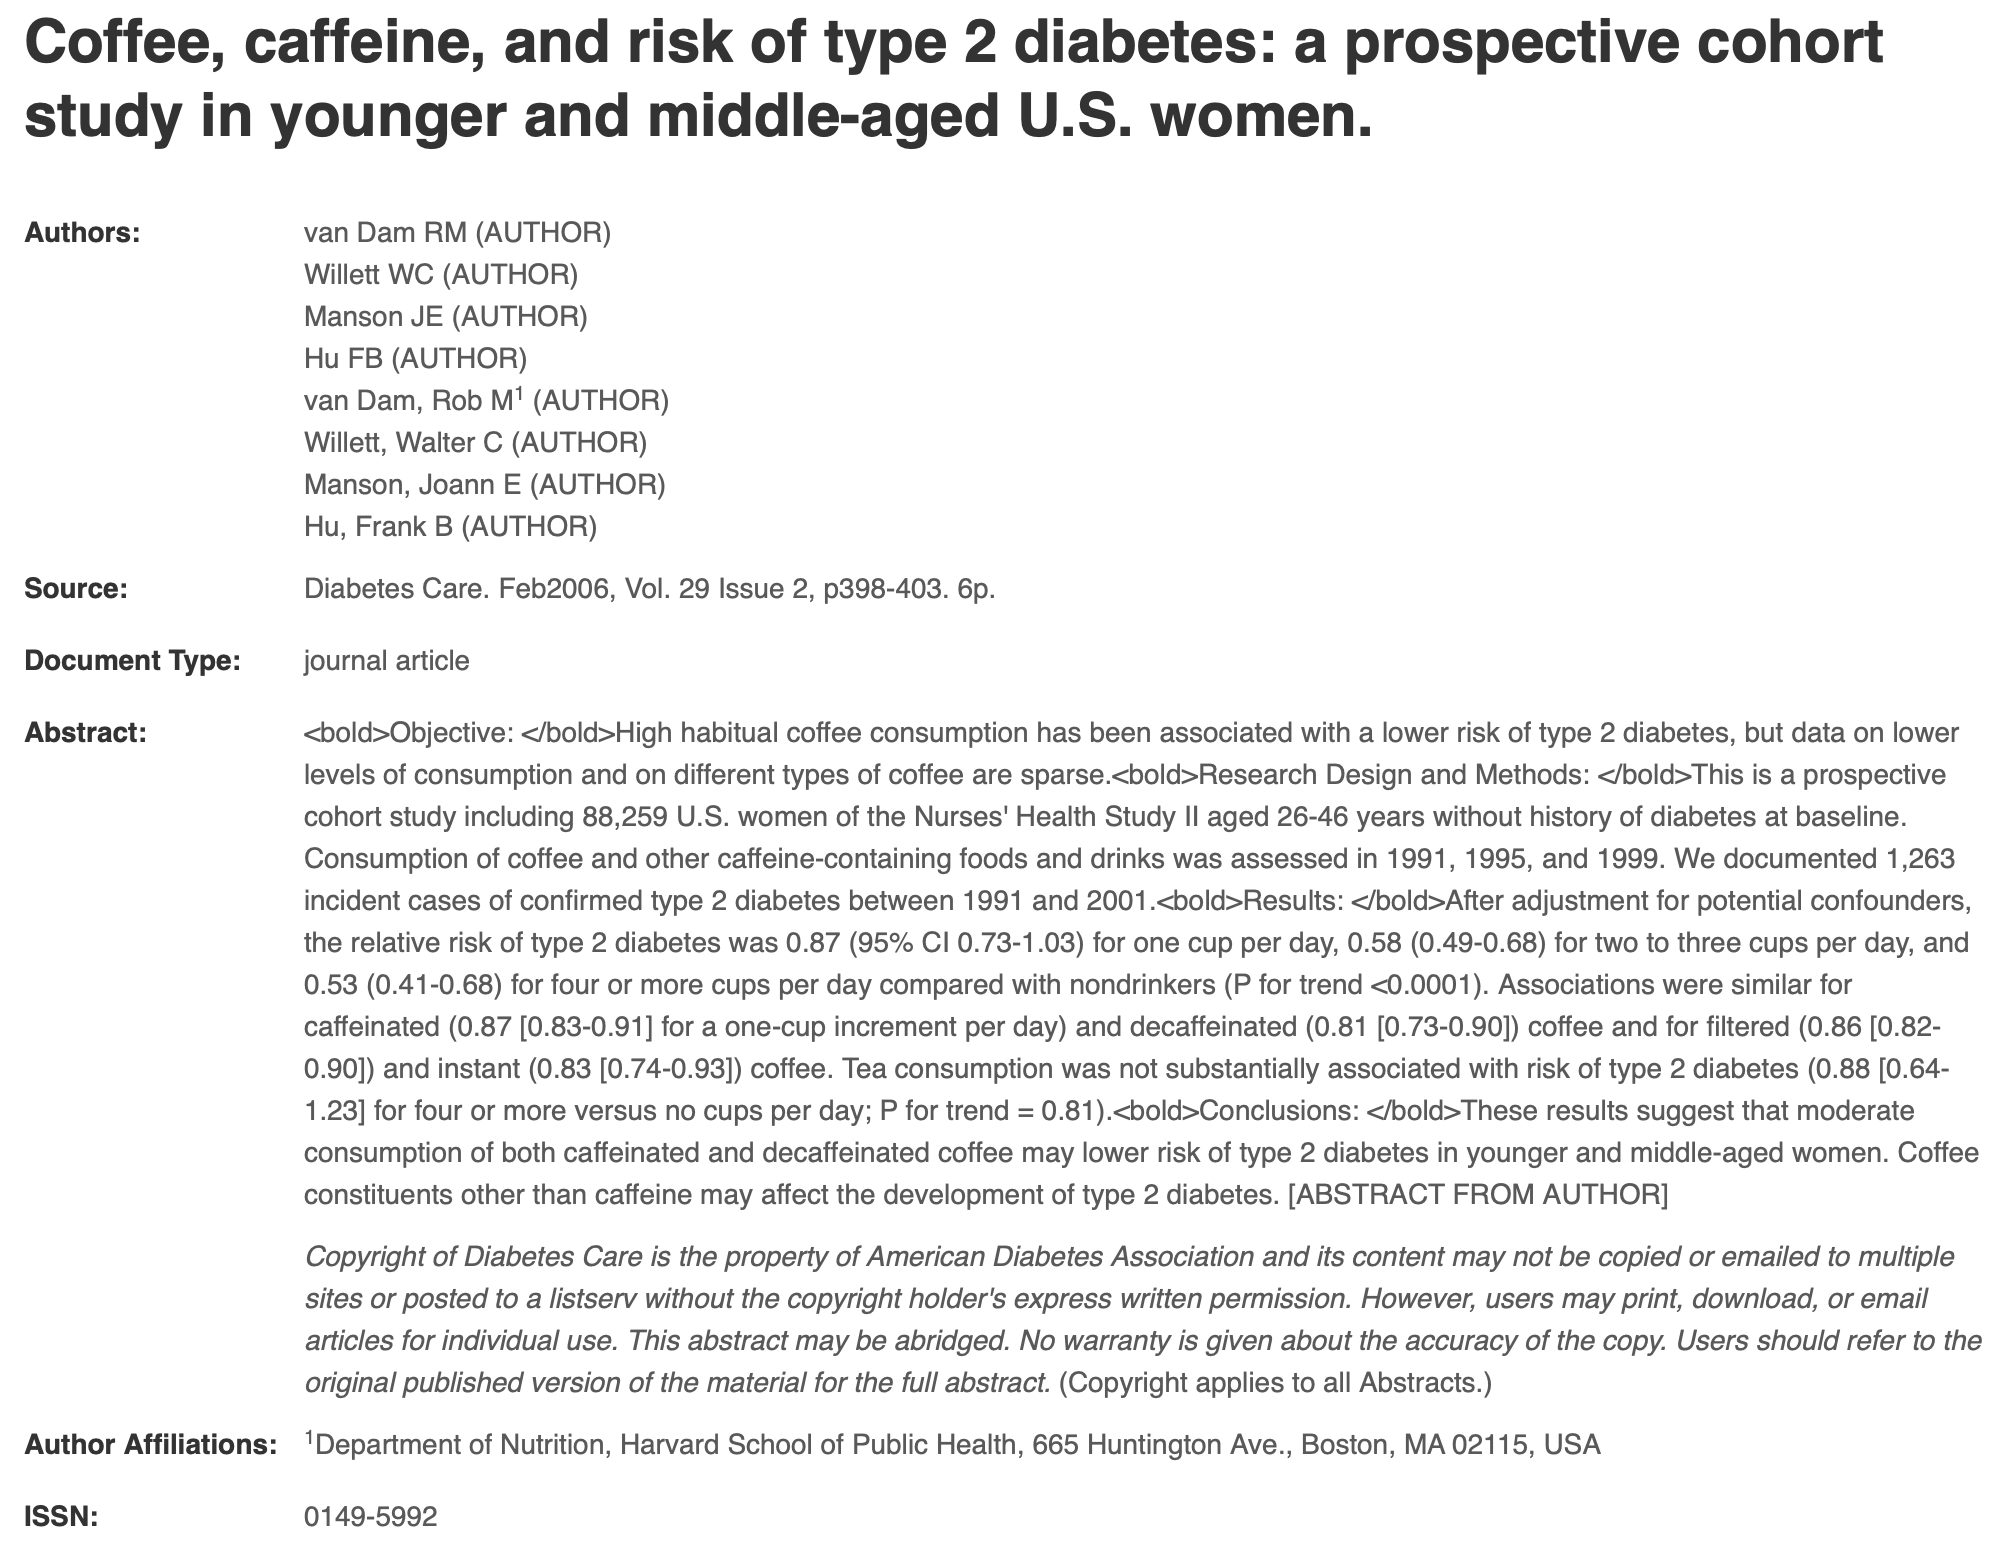
\includegraphics[width=.9\linewidth]{/Users/shauryasingh/org/.attach/33/262aa9-0c25-4bd7-9725-6a4075ccd95d/_20211026_192803Mellitus.png}
\end{center}

\subsection{MLA Citation}
\label{sec:org6a78a88}
\begin{quote}
Alperet, Derrick, et al. “1575-P: Influence of Adolescent and Maternal Coffee Consumption on Risk of Obesity and Type 2 Diabetes Mellitus in Middle-Aged Women and Their Offspring: Results from Two Prospective Cohort Studies in the United States.” Diabetes, vol. 68, no. Supplement 1, June 2019, pp. 1575-P. DOI.org (Crossref), \url{https://doi.org/10.2337/db19-1575-P}.
\end{quote}
\subsection{A brief summary of the text}
\label{sec:org20180ba}
In a double-blind randomized trial, coffee intake was shown to decrease fat mass in healthy overweight adults. This suggests that coffee could be modulating lower type 2 diabetes mellitus (T2DM) risk among adults through pathways involving adiposity. It is not known if earlier-life exposure to coffee intake could modulate risk of developing childhood obesity and, ultimately, T2DM later in life. Adolescent caffeinated coffee intake was associated with 17\% lower T2DM risk
\subsection{Comment on the authority or credibility of the author;}
\label{sec:org9cdb703}
The authors are graduate students from reputable institutions (such as harvard) and years of experience in their respective fields. The journal itself is reputable, as it is the American Diabetes Association, one of the largest diabetic organizations and journals worldwide. Therefore, the source is trustworthy.
\subsection{Comment on strengths and weaknesses of their argument;}
\label{sec:org9232a67}
While they did a good job of keeping the experiment controlled and reporting results, even they mentioned there are/were possible factors that could play into this, one of the main issues being exposure to coffee in earlier life (pre-utero/pre-teen).
\subsection{The author’s point of view; and}
\label{sec:org97b5904}
The author is a neutral writer, in that this is a purely informative piece
\subsection{How the text relates to your question or thesis.}
\label{sec:orge5b1a55}
The text identifies Adolescent as well as Maternal Coffee intake and relates it risk with a risk of diabetes in elder women. While my research focuses on adolescents, the research paper provides insight and data that will be useful.
\section{Article 3: Role of coffee in modulation of diabetes risk}
\label{sec:orgd8dc712}
\subsection{PDF}
\label{sec:orgbbed07d}
\begin{center}
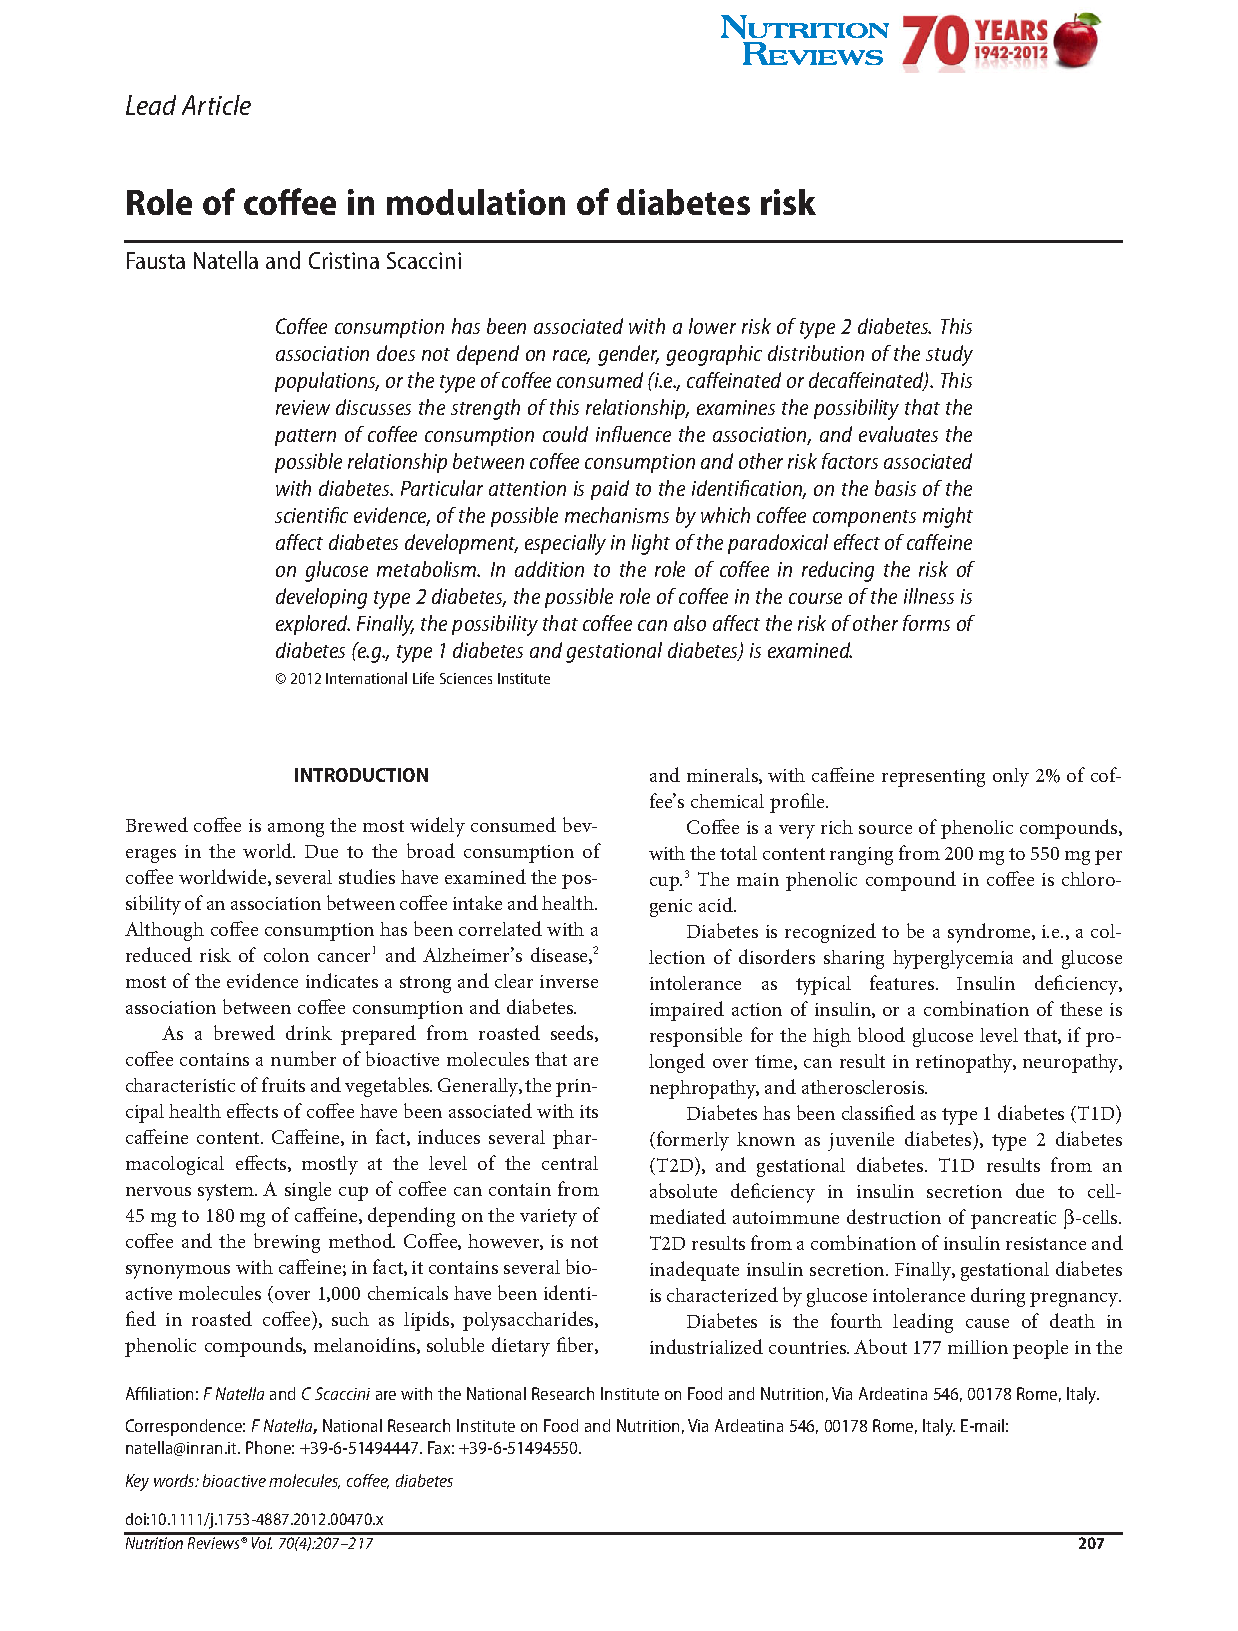
\includegraphics[width=.9\linewidth]{./citations/RoleOfCoffeeIn.pdf}
\end{center}
\subsection{MLA Citation}
\label{sec:org9c0edc5}
\begin{quote}
Natella, Fausta, and Cristina Scaccini. “Role of Coffee in Modulation of Diabetes Risk.” Nutrition Reviews, vol. 70, no. 4, Apr. 2012, pp. 207–17. DOI.org (Crossref), \url{https://doi.org/10.1111/j.1753-4887.2012.00470.x}.
\end{quote}
\subsection{A brief summary of the text}
\label{sec:org7fa0d85}
Coffee consumption has been associated with a lower risk of type 2 diabetes. This review examines the strength of this relationship, examines the possibility that the pattern of coffee consumption could influence the association, and evaluates the possible relationship between coffee consumption and other risk factors associated with diabetes. Particular attention is paid to the identification of the possible mechanisms by which coffee components might affect diabetes development.
\subsection{Comment on the authority or credibility of the author;}
\label{sec:org06f9ea7}
The author has previous experience in the topic but not as much as some of the other articles. The publisher is also not the most reputable, and the writing is informal at times.
\subsection{Comment on strengths and weaknesses of their argument;}
\label{sec:orge7ea0c6}
The author provides a good background as to why coffee is an issue and what are the effects of coffee. However, the author does not visualize data very well, and doesn't provide much original information. The article may be used as a reference for statistics on coffee, but should be used as a reputable source.
\subsection{The author’s point of view; and}
\label{sec:orgce941b8}
The author is a neutral writer, in that this is a purely informative piece
\subsection{How the text relates to your question or thesis.}
\label{sec:orga8b707d}
My research relates to coffee consumption and the risk of Diabetes. While this article doesn't focus on any age groups, it provides accurate data on the results of coffee on diabetes risk
\section{Article 4:  Coffee Consumption and Risk of Type 2 Diabetes Mellitus Among Middle-aged Finnish Men and Women.}
\label{sec:orgbd8c2fc}
\subsection{PDF\hfill{}\textsc{ATTACH}}
\label{sec:org303d1b6}
\begin{center}
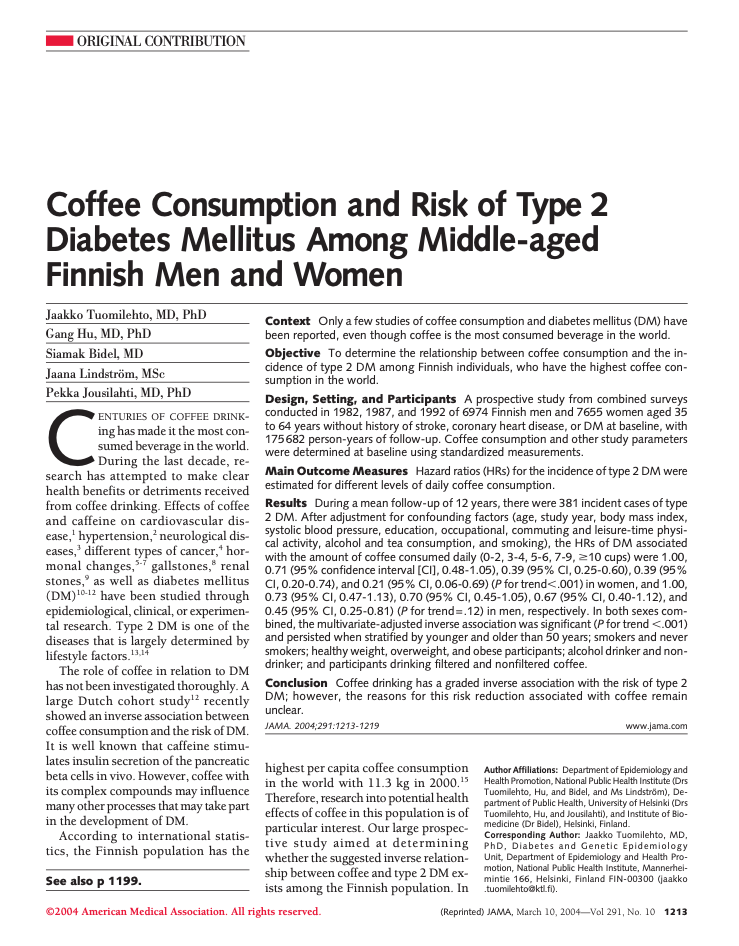
\includegraphics[width=.9\linewidth]{/Users/shauryasingh/org/.attach/56/e9ffbb-c7cf-4cda-8bf1-5be79084552e/_20211026_191341Finnish.png}
\end{center}

\subsection{MLA Citation}
\label{sec:orgcecc063}
\begin{quote}
Tuomilehto, Jaakko, et al. “Coffee Consumption and Risk of Type 2 Diabetes Mellitus Among Middle-Aged Finnish Men and Women.” JAMA: Journal of the American Medical Association, vol. 291, no. 10, Mar. 2004, pp. 1213–1219. EBSCOhost, doi:10.1001/jama.291.10.1213.
\end{quote}
\subsection{A brief summary of the text}
\label{sec:orgd979969}
Finnish individuals have the highest coffee consumption in the world. Coffee consumption and other study parameters were determined at baseline using standardized measurements. After adjustment for confounding factors (age, study year, body mass index, systolic blood pressure, education, occupational, commuting and leisure-time physical activity, alcohol and tea consumption, and smoking), the HRs of DM associated with the amount of coffee consumed daily (0-2, 3-4, 5-6, 7-9,  10 cups) were 1.00, 0.71 (95\% confidence interval [CI], 0.48-1.05) (P for trend=.001). In both sexes, the multivariate-adjusted inverse association was significant. The author concluded Coffee drinking has a graded inverse association with the risk of type 2 DM; however, the reasons for this risk reduction associated with coffee remain unclear.
\subsection{Comment on the authority or credibility of the author;}
\label{sec:orgac71651}
Professor Jaakko Tuomilehto qualified as MD in 1973 and MA in sociology in 1975 and PhD in Epidemiology and Public Health in 1975. He is currently working as the Chief Scientific Officer at Dasman Diabetes Institute in Kuwait. He is well known for his expertise in the subject.
\subsection{The author’s point of view; and}
\label{sec:org447e950}
The author is a neutral writer, in that this is a purely informative piece
\subsection{How the text relates to your question or thesis.}
\label{sec:org280e45f}
Once again, my research relates to coffee consumption and the risk of Diabetes. While this article doesn't focus on any age groups, it provides accurate data on the results of coffee on diabetes risk. Finland, a country very dependant on coffee, can also show us how socioconomic factors play into coffee consumption.
\section{Article 5: Coffee consumption is inversely associated with type 2 diabetes in Chinese.}
\label{sec:org1edae3c}
\subsection{PDF}
\label{sec:orgaae1209}
\begin{center}
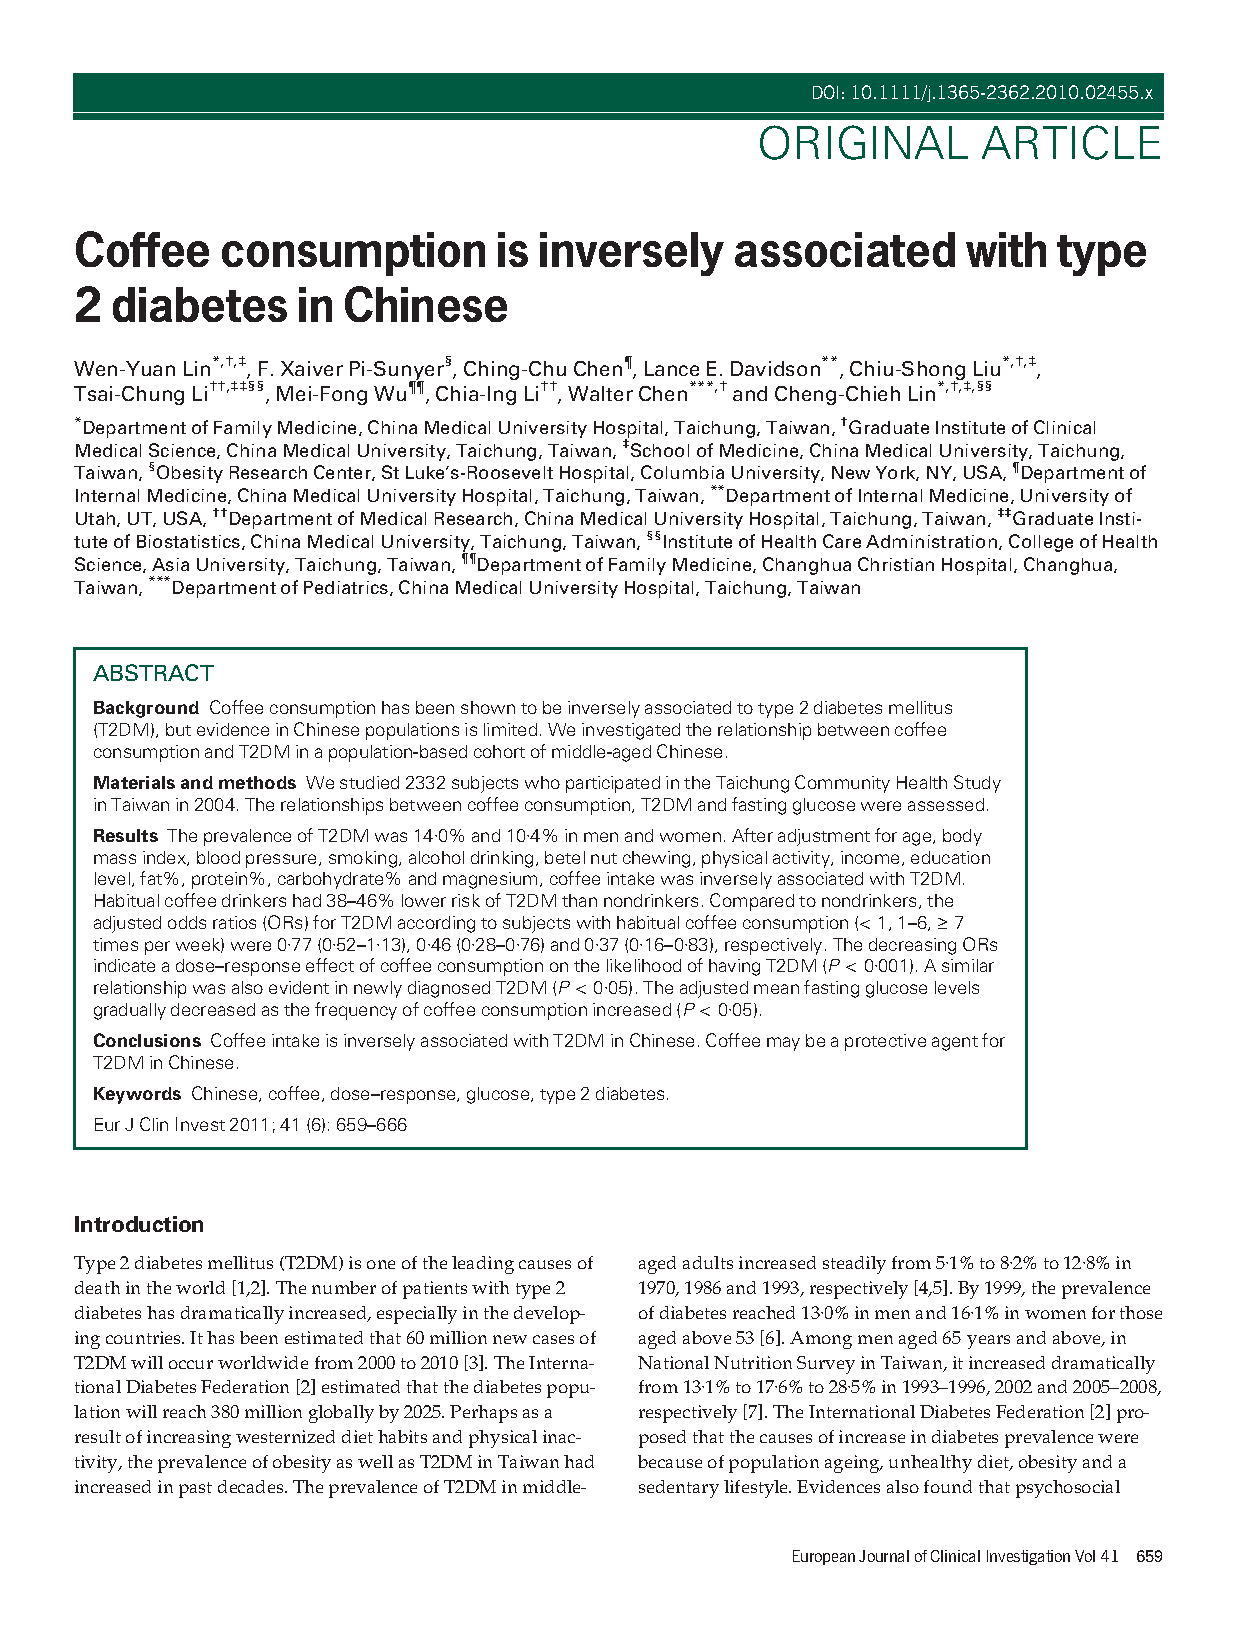
\includegraphics[width=.9\linewidth]{./citations/CoffeeInverseChinese.pdf}
\end{center}
\subsection{MLA Citation}
\label{sec:org8dc4924}
\begin{quote}
Lin, Wen-Yuan, et al. “Coffee Consumption Is Inversely Associated with Type 2 Diabetes in Chinese.” European Journal of Clinical Investigation, vol. 41, no. 6, June 2011, pp. 659–666. EBSCOhost, doi:10.1111/j.1365-2362.2010.02455.x.
\end{quote}
\subsection{A brief summary of the text}
\label{sec:orgb3d1021}
Coffee consumption has been shown to be inversely associated to type 2 diabetes mellitus (T2DM), but evidence in Chinese populations is limited. They investigated the relationship between coffee consumption and T2DM in a population-based cohort of middle-aged Chinese. After adjustment for age, body mass index, blood pressure, smoking and other factors, coffee intake was  inversely associated with t2DM. Habitual coffee drinkers had 38-46\% lower risk of T2 DM than nondrinkers.
\subsection{Comment on the authority or credibility of the author;}
\label{sec:org6916335}
Wen-yuan Lin is a Research Chemist at ToKai Carbon CB, and is experienced in the topic. He also has other reputable articles published to well known journals such as Nature.
\subsection{Comment on strengths and weaknesses of their argument;}
\label{sec:org5f72897}
The author is purely alternative, and presents data in a well thought out manner. There is no argument, and the author summarises and analysis the data well.
\subsection{The author’s point of view; and}
\label{sec:orgd29729e}
The author is a neutral writer, in that this is a purely informative piece
\subsection{How the text relates to your question or thesis.}
\label{sec:org7a951b9}
Similar to the previous 3, this supports my hypothesis that coffee consumption may be beneficial for middle aged men and women,
\section{Article 6: Increased coffee, tea, or other sugar-sweetened beverage consumption in adolescents is associated with less satisfactory dietary quality, body fatness and serum uric acid profiles over the past 18 years in Taiwan.}
\label{sec:org66f2c43}
\subsection{PDF\hfill{}\textsc{ATTACH}}
\label{sec:org72d3cd2}
\begin{center}
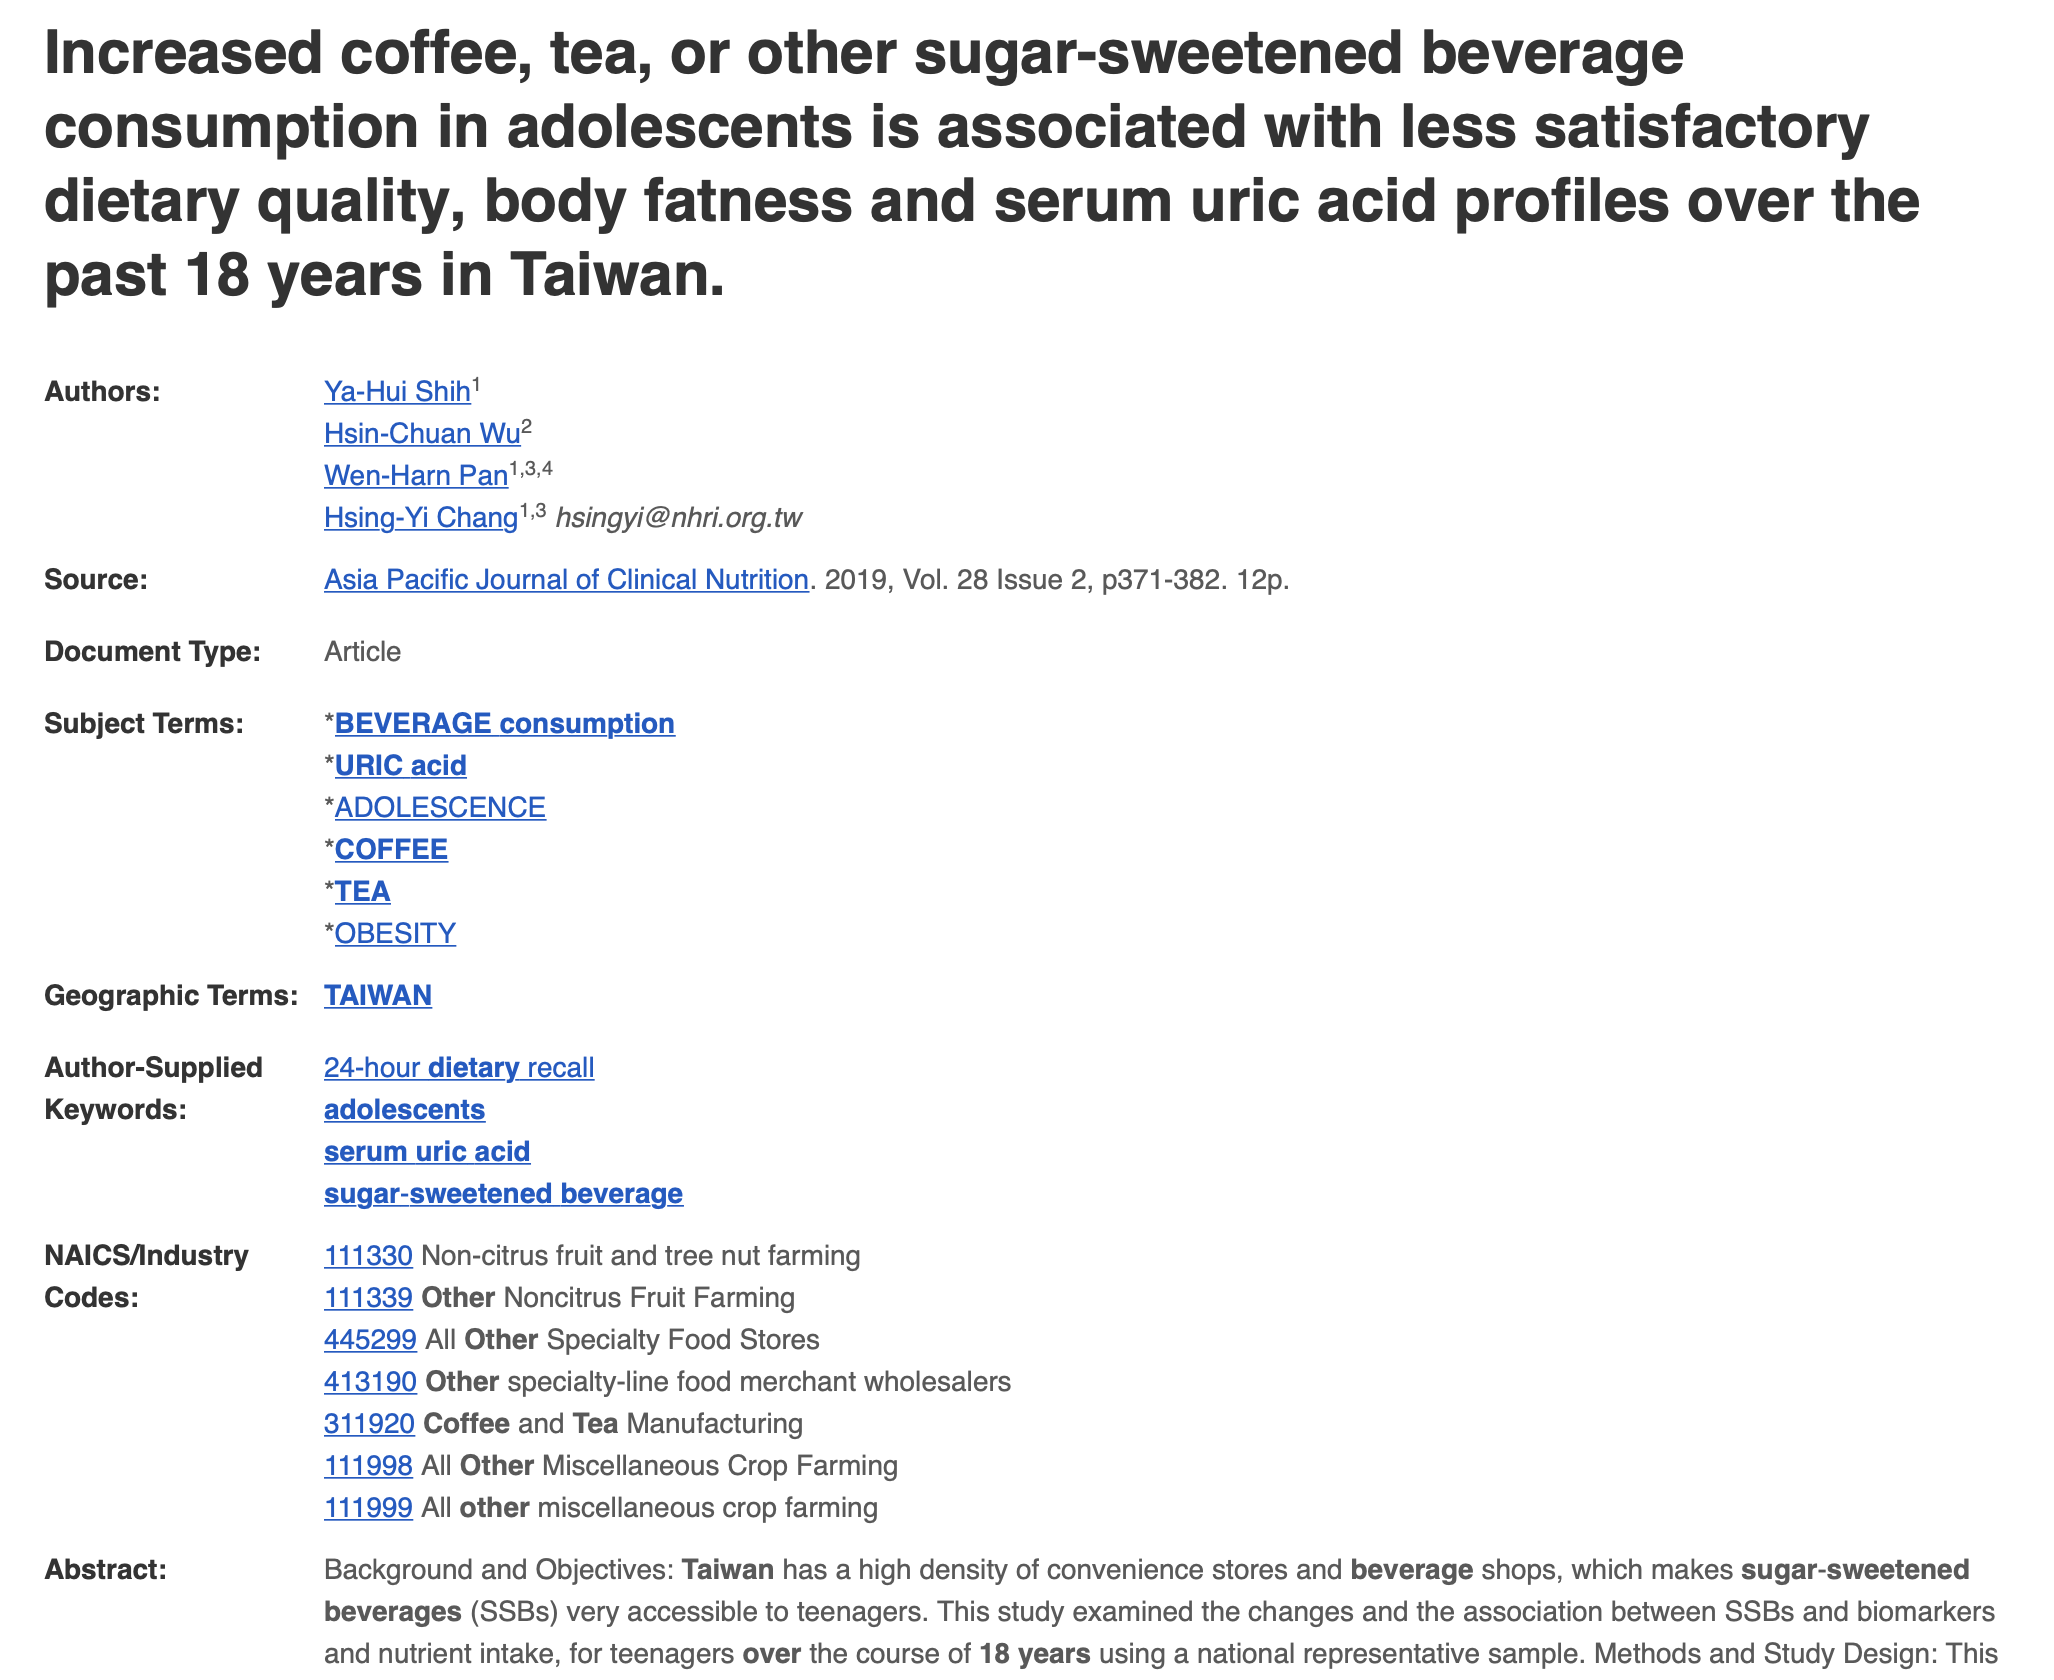
\includegraphics[width=.9\linewidth]{/Users/shauryasingh/org/.attach/d0/9b3015-3ae5-4b1c-a7c4-6dbe9a7f0603/_20211026_193127CoffeeFatVietnam.png}
\end{center}

\subsection{MLA Citation}
\label{sec:orga3d5676}
\begin{quote}
Ya-Hui Shih, et al. “Increased Coffee, Tea, or Other Sugar-Sweetened Beverage Consumption in Adolescents Is Associated with Less Satisfactory Dietary Quality, Body Fatness and Serum Uric Acid Profiles over the Past 18 Years in Taiwan.” Asia Pacific Journal of Clinical Nutrition, vol. 28, no. 2, Apr. 2019, pp. 371–382. EBSCOhost, doi:10.6133/apjcn.201906\_28(2).0020.
\end{quote}
\subsection{A brief summary of the text}
\label{sec:orgb52c5e1}
Taiwan has a high density of convenience stores and beverage shops, which makes sugar-sweetened beverages (SSBs) very accessible to teenager. This study examined the changes and the association between SSBs and biomarkers and nutrient intake, for teenagers over the course of 18 years. Intake of coffee or tea increased significantly in the 18 years of this study (p<0.01), whereas intake of SSBs decreased significantly (p=0.05). Intake was significantly higher among second survey participants and those with high total energy intakes.
\subsection{Comment on the authority or credibility of the author;}
\label{sec:org2c471fa}
Ya-Hui Shih is a student at the National Health Research Institutes, Division of Preventive Medicine and Health Service Research. He has multiple other papers published to reputable journals, and is an expert in evidence-based-medicine.
\subsection{Comment on strengths and weaknesses of their argument;}
\label{sec:org83ee203}
The article is slightly vague, and lacks proper control of the experiment. The methodology could be better, and the experiment could be fine tuned to further eliminate human error. I will likely use this source to write about the cultural aspect of coffee consumption in adolescents
\subsection{The author’s point of view; and}
\label{sec:orgcb61a42}
The author is a neutral writer, in that this is a purely informative piece
\subsection{How the text relates to your question or thesis.}
\label{sec:org91109ae}
Once again, my research relates to coffee consumption and the risk of Diabetes. While this article doesn't focus on any age groups, it provides accurate data on the results of coffee on diabetes risk. Similar to Finland, the issue with Taiwan is that coffee is very accessible, similar to America. This raises issues with early onset coffee addiction in adolescents, something I want to study in my paper.
\section{Article 7: Weight Gain in Older Adolescent Females: The Internet, Sleep, Coffee, and Alcohol}
\label{sec:org14a53ed}
\subsection{PDF}
\label{sec:orgeb93ada}
\begin{center}
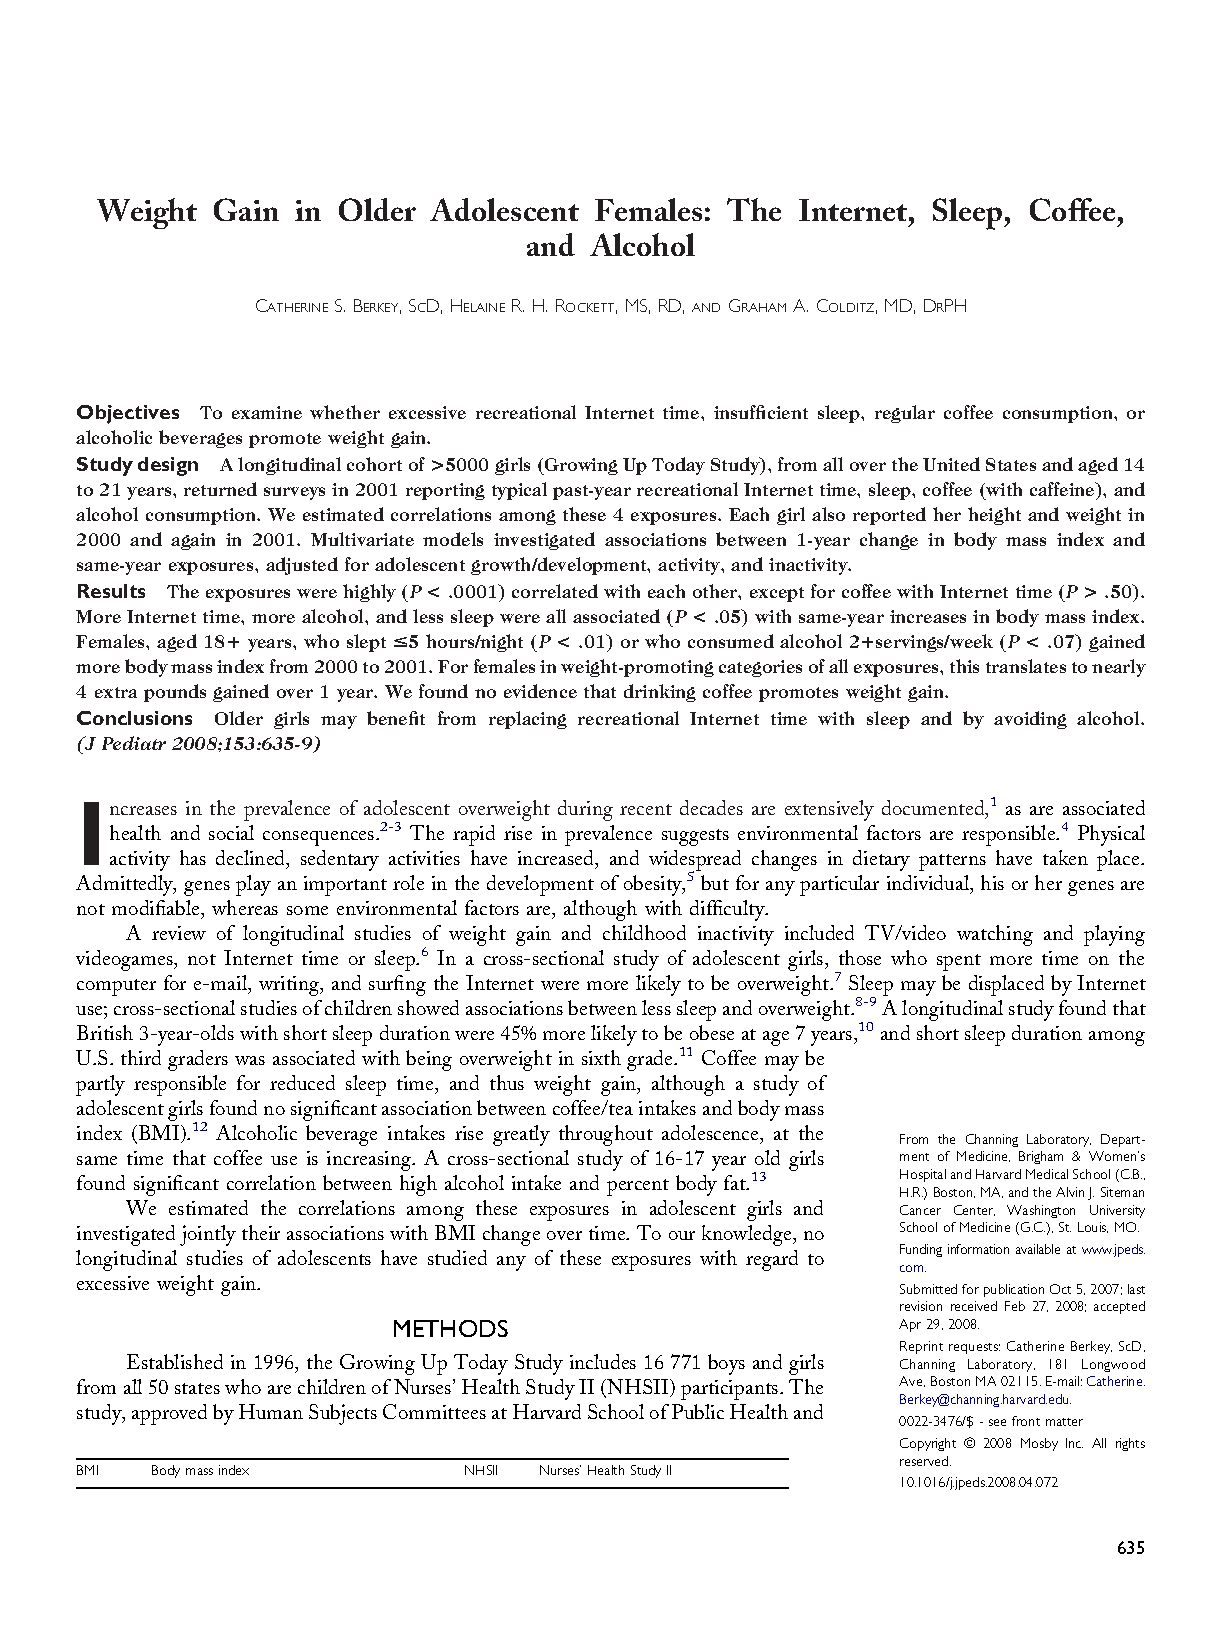
\includegraphics[width=.9\linewidth]{./citations/WeightGainIn.pdf}
\end{center}
\subsection{MLA Citation}
\label{sec:org58b0a2b}
\begin{quote}
Berkey, Catherine S., et al. “Weight Gain in Older Adolescent Females: The Internet, Sleep, Coffee, and Alcohol.” The Journal of Pediatrics, vol. 153, no. 5, Nov. 2008, pp. 635-639.e1. DOI.org (Crossref), \url{https://doi.org/10.1016/j.jpeds.2008.04.072}.
\end{quote}
\subsection{A brief summary of the text}
\label{sec:orgc56d901}
More Internet time, more alcohol, and less sleep were all associated with same-year increases in body mass index. The exposures were highly (P <.0001) correlated with each other, except for coffee with Internet time (P >.50). Older girls may benefit from replacing recreational Internet time with sleep and by avoiding alcohol. Younger girls may benefit from avoiding both alcohol and coffee.
\subsection{Comment on the authority or credibility of the author;}
\label{sec:org4d445bd}
Catherine S. Berkey, DSc is a Research Associate in Medicine at Brigham and Women's Hospital and Harvard Medical School. She is a well-known expert in her field, and has done similar studies in the past. She has multiple studies published to reputable peer-reviewed journals
\subsection{Comment on strengths and weaknesses of their argument;}
\label{sec:org880dc0d}
The information in the article is outdated, and internet usage has likely changed since then. Additionally, the data is not properly presented, with a lack of visuals. I would like to replace this source in the future, with one of a similar idea but with newer and better visualized data.
\subsection{The author’s point of view; and}
\label{sec:orga2c28c2}
The author is a neutral writer, in that this is a purely informative piece
\subsection{How the text relates to your question or thesis.}
\label{sec:org3094f7b}
Similar to Taiwan, the issue is that coffee is very accessible, similar to America. This raises issues with early onset coffee addiction in adolescents. Additionally, the internet can amplify this behavior, sleeping late and drinking coffee is an unnoticed detrimental sideeffect of adolescent coffee culture, something I want to study in my paper.
\end{document}
